\documentclass[letterpaper]{article} 

\usepackage{amssymb,amsmath} 
\usepackage{graphicx}
\usepackage[section]{placeins}
\usepackage{perpage}
\MakePerPage{footnote}


\begin{document}
\title{STA 511 Homework \#3}
\date{October 22 2015}
\author{Suruchi Jaikumar Ahuja}
\maketitle

\begin{enumerate}

\item The density on [0,$\infty$) is given by 
\begin{equation*}
          f(x)=\dfrac{2}{\pi(1+x) \sqrt{x^2+2x}}
\end{equation*}\\

The dominating curve is given by\\
\begin{equation*}
c_{\theta} g_{\theta}(x)=
\begin{cases}
\frac{2}{\pi \sqrt(2x)} & 0 \leq x \leq \theta\\
\frac{2}{\pi x^2} & x \geq \theta\\
\end{cases}
\end{equation*}

\begin{enumerate}

\item 	To prove $0 \leq x \leq \theta $
\begin{equation*}
\dfrac{f(x)}{c_{\theta}g_{\theta}} =\dfrac{\dfrac{2}{\pi(1+x) \sqrt{x^2+2x}}}{\dfrac{2}{\pi\sqrt{2x}}}
\end{equation*}\\

Since the numerators are same , they can be ignored and the remaining equation is now considered,which leaves us with;\\

\begin{equation*}
\dfrac{f(x)}{c_{\theta}g_{\theta}} =\dfrac{\sqrt{2x}} {(1+x)\sqrt{x^2+2x}}
\end{equation*}\\

 For every value of $x > 0$ in $ \dfrac{f(x)}{c_{\theta}g_{\theta}}$ ; the denominator is greater than the numerator,\\

So $\dfrac{f(x)}{c_{\theta} g_{\theta}} \leq 1 $\\\\

$\Rightarrow f(x) \leq c_{\theta} g_{\theta}$\\

Now to prove $ x > \theta $ \\
\begin{equation*}
\dfrac{f(x)}{c_{\theta}g_{\theta}} =\dfrac{\dfrac{2}{\pi(1+x) \sqrt{x^2+2x}}}{\dfrac{2}{\pi x^2}}
\end{equation*}\\

Since the numerators are same , they can be ignored and the remaining equation is now considered,which leaves us with;\\

\begin{equation*}
\dfrac{f(x)}{c_{\theta}g_{\theta}} = \dfrac {x}{(1+x)\sqrt{x^2+2x}}
\end{equation*}

 For every value of $x > 0$ in $ \dfrac{f(x)}{c_{\theta}g_{\theta}}$ ; the denominator is greater than the numerator,\\

So $\dfrac{f(x)}{c_{\theta} g_{\theta}} \leq 1 $\\\\

$\Rightarrow f(x) \leq c_{\theta} g_{\theta}$\\

Hence the $  f(x) \leq c_{\theta} g_{\theta} $ stands true for both conditions \\



\item To show that $c_{\theta}$ is minimal for $\theta=2^{\frac{1}{3}}$\\

\begin{equation*}
\Rightarrow \int_{0}^{\theta}\dfrac{2}{\pi \sqrt{2x}}+\int_{\theta}^{\infty}\dfrac{2}{\pi x^2}
\end{equation*}\\

\begin{equation*}
\rightarrow\left.\frac{4\sqrt{x}}{\pi}\right|_0^\theta -\left.\frac{2}{\pi x}\right|_\theta^\infty
\end{equation*}\\

\begin{equation*}
\rightarrow\dfrac{4 \theta^{\frac{1}{2}}}{\pi}+\dfrac{2}{\pi \theta}
\end{equation*}\\

\begin{equation*}
\rightarrow\dfrac{dc(\theta)}{d \theta} = \dfrac{2}{\pi \sqrt{2 \theta}}-\dfrac{2}{\pi \theta^2}
\end{equation*}\\

On simplifying the above equation and substituting $\theta = 2^{\frac{1}{3}}$, we get\\

\begin{equation*}
\Rightarrow\dfrac{2}{\pi}[2^{-\frac{2}{3}}-2^{-\frac{2}{3}}] \rightarrow 0
\end{equation*}\\


\item 
Here $\theta = 2^{1/3}$ and 
the dominating curve is given by\\
\begin{equation*}
c_{\theta} g_{\theta}(x)=
\begin{cases}
\frac{2}{\pi \sqrt(2x)} & 0 \leq x \leq \theta\\
\frac{2}{\pi x^2} & x \geq \theta\\
\end{cases}
\end{equation*}
 
 So now on integrating the $c_\theta g_\theta$, we get c = $\dfrac{(3*2^{2/3})}{\pi}$\\
 Now the generalized rejection method is performed on the obtained 500 observations from f(x)\\
 A histogram of the accepted observations with the pdf f superimposed is constructed (Refer to Figure 1).\\
 \begin{figure}[h]
    \centering
     \includegraphics[scale=0.45]{figure.jpeg}
      \caption{ Histogram of accepted observations with the pdf f superimposed on it }
        \label{Figure 1}
\end{figure}\\

\end{enumerate} 

\item   The Laplace distribution has pdf f(x) given by\\

\begin{equation*}
f(x) =\dfrac{\theta}{2}e^{-\theta |x|}  for \theta >0  and for  -\infty <x <\infty
\end{equation*}

\begin{enumerate}
\item Here we assume \\
$\theta =1$\\
$\mu =3 $\\
\begin{equation*}
g(x)=\dfrac{\mu}{\pi(\mu^2 + x^2)}
\end {equation*}\\

To find the optimal rejection constant c we use the formula
\begin{equation*}
\Rightarrow c=sup\dfrac{f(x)}{g(x)}
\end{equation*}\\

\begin{equation*}
\rightarrow c = \dfrac{\dfrac{\theta}{2}e^{-\theta |x|}}{\dfrac{\mu}{\pi(\mu^2 + x^2)}}
\end{equation*}\\

\begin{equation*}
\rightarrow c= \dfrac{\dfrac{1}{2} e^-|x|}{\dfrac{3}{\pi}(9+x^2)}
\end{equation*}\\

\begin{equation*}
\rightarrow c = \dfrac{\pi}{6}e^{-|x|}(9+x^2)
\end{equation*}\\

\begin{figure}[h]
    \centering
     \includegraphics[scale=0.45]{2a.jpeg}
      \caption{ Optimal rejection constant c-Maximum value }
        \label{Figure 2}
\end{figure}


\begin{verbatim}
x = seq(-10,10,length=1000)
y = pi/6*exp(-abs(x))*(9+x^2)
plot(x,y)
\end{verbatim}

\item Algorithm for generating random variables from the Cauchy distribution with the optimal parameter value for $\mu=3$ using Uniform(0,1) random variables.\\
Consider Y = F (x)\\
$\rightarrow$ x =$ F^{-1}$(Y)\\
\begin{equation*}
 F = \dfrac{1}{\pi} \arctan(x) + \dfrac{1}{2}
\end{equation*}

\begin{equation*}
 x =\tan(\pi(y-\dfrac{1}{2}))
\end{equation*}

For F(x;$\mu$,c)
\begin{equation*}
\rightarrow \dfrac{1}{\pi}\arctan(\dfrac{x-\mu}{c})-\dfrac{1}{2}
\end{equation*}

Step 1: In this case the first step is to generate U from Uniform(0,1)\\
Step 2: First we have 
\begin{equation*}
g(x)=\dfrac{\mu}{\pi(\mu^2 + x^2)}
\end {equation*}\\
 
\begin{equation*}
 G(x) = \int_{-\infty}^{x} \dfrac{\mu}{\pi(\mu^2+ z^2)} dz
\end{equation*}\\

\begin{equation*}
\rightarrow \dfrac{1}{\mu \pi}\int_{-\infty}^{x}\dfrac{1}{1+\dfrac{z^2}{\mu^2}} dz
\end{equation*}\\

\begin{equation*}
 G(x) = \mu = \dfrac{1}{\pi} \tan ^{-1}(\dfrac{x}{\mu})+\dfrac{\pi}{2}
\end{equation*}\\

\begin{equation*}
\rightarrow \mu = \dfrac{1}{\pi} \tan^{-1}(\dfrac{x}{\mu}) + \dfrac{\pi}{2}
\end{equation*}\\

\begin{equation*}
\Rightarrow x= \mu \tan[\pi(\mu-\dfrac{1}{2})]
\end{equation*}\\



\item Using a generalized rejection algorithm, 1000 observations are generated from the Laplace distribution($\theta = 1$)\\
A histogram of the accepted observations with the pdf of the Laplace distribution was constructed.(Refer to Figure 3)
\begin{figure}[h]
    \centering
     \includegraphics[scale=0.45]{cauchy.jpeg}
      \caption{ Histogram of xc[t1$\leq$ 1] }
        \label{Figure 3}
\end{figure}


\textbf {R Code}\\
\begin{verbatim}
x=seq(-10,10,length=1000)
c <- (pi/6)*exp(-abs(x))*(9+x^2)#optimal rejection constant
xc <- rcauchy(1000,0,1) # generating 1000 observations
n <- runif(1000,0,1)

fun <- function(x)
{
  s<- (6/(pi*(9+x^2)*exp(-abs(x))))
}
t <- c*sapply(xc, fun)
t1 <- n*t

hist(xc[t1<=1],prob=T,ylim=c(0,0.5))

laplace <- function(x)
{
  f<- (1/2)*(exp(-abs(x)))
}

lines(x,laplace(x))
sum(t1<=1)/1000
\end{verbatim}
 
 \textbf{ OUTPUT:} \\
The acceptance percentage is 84.8 percent\\\\


\end{enumerate}


\item The beta distribution wih parameters $ \alpha > 0 $ and $\beta >0 $ has a continuous density given by \\
\begin{equation*}
f(x) = \dfrac{1}{B(\alpha , \beta)}x^{\alpha-1}(1-x)^{\beta -1} for 0<x<1
\end{equation*}\\

\begin{enumerate}

\item 
 To make plots in R of the target density when $(\alpha,\beta)$= (0.5, 0.5),(1, 0.5),(0.5, 1),(1, 1),(2, 2),(5, 10)\\
Refer to Figure 4 for the plots of target density\\
\begin{figure}[h]
    \centering
     \includegraphics[scale=0.5]{hw3.jpeg}
      \caption{ Plots to show target density when $(\alpha,\beta)$= (0.5, 0.5),(1, 0.5),(0.5, 1),(1, 1),(2, 2),(5, 10) \label{overflow}}
      \label{Figure 4}
\end{figure}

\textbf {R Code :}\\
\begin{verbatim}
x = seq(0.1,1,300)
a1=0.5; a2=1; a3=0.5; a4=1; a5=2; a6=5;
b1=0.5; b2=0.5; b3=1 ;b4=1; b5=2; b6=10

f=function(x){
  gamma(a1+b1)/(gamma(a1)*gamma(b1))*x^(a1-1)*(1-x)^(b1-1)
  }
f2=function(x){
  gamma(a2+b2)/(gamma(a2)*gamma(b2))*x^(a2-1)*(1-x)^(b2-1)
  }
f3=function(x){
  gamma(a3+b3)/(gamma(a3)*gamma(b3))*x^(a3-1)*(1-x)^(b3-1)
  }
f4=function(x){
  gamma(a4+b4)/(gamma(a4)*gamma(b4))*x^(a4-1)*(1-x)^(b4-1)
  }
f5=function(x){
  gamma(a5+b5)/(gamma(a5)*gamma(b5))*x^(a5-1)*(1-x)^(b5-1)
  }
f6=function(x){
  gamma(a6+b6)/(gamma(a6)*gamma(b6))*x^(a6-1)*(1-x)^(b6-1)
  }

plot(x, f(x), type="l", col=1)
lines(x,f2(x),type="l",col=2)
lines(x,f3(x),type="l",col=3)
lines(x,f4(x),type="l",col=4)
lines(x,f5(x),type="l",col=5)
lines(x,f6(x),type="l",col=6)
legend("topright",lwd =c(2,2,2,2,2,2),
legend = c("f(x)=f","f2(x)=f2","f3(x)=f3","f4(x)=f4","f5(x)=f5","f6(x)=f6"),
col=c(1,2,3,4,5,6))
\end{verbatim}



\item Let $\alpha > 1$ and $\beta > 1 $ \\
\begin{equation*}
f(x) = \dfrac{1}{B(\alpha , \beta)}x^{\alpha-1}(1-x)^{\beta -1} for 0<x<1
\end{equation*}\\
 
 On differentiating the f(x) equation ,\\
 \begin{equation*}
 \rightarrow \dfrac{df}{dx} =\dfrac{1}{ B(\alpha,\beta) } x^{\alpha-2}(1-x)^{\beta-1}-\dfrac{1}{ B(\alpha,\beta) } x^{\alpha-1}(1-x)^{\beta-2}
 \end{equation*}\\

  Now taking all the terms common in one side and simlifying the above equation;\\
  \begin{equation*}
\rightarrow \dfrac{df}{dx} =\dfrac{1}{B(\alpha,\beta)} x^{\alpha-2}(1-x)^{\beta-2} [(1-x)(\alpha -1 )-(\beta-1)x]
\end{equation*}\\


Using the second part of the equation and simplifying it further we get \\

[(1-x)($\alpha$ -1)-($\beta$-1)x]\\ = [($\alpha$ - 1) -x($\alpha$ -1) - x($\beta$ - 1)]\\
                        =[($\alpha$-1)-x[($\alpha$-1)+($\beta$-1)]\\
                          =($\alpha$)-x[($\alpha+\beta$)-2]\\\\

Now substituting the [(1-x)($\alpha$ -1)-($\beta$-1)x] in $\dfrac{df}{dx}$;   \\

$\rightarrow \dfrac{1}{B(\alpha,\beta)} x^{\alpha-2}(1-x) [(\alpha+\beta)-2] [\dfrac{(\alpha-1)}{(\alpha+\beta-2)}-x]$\\

Considering only $ [\dfrac{(\alpha-1)}{(\alpha+\beta-2)}-x]$\\

The equation can be re written as \\
\begin{equation*}
x \leq \dfrac{(\alpha-1)}{((\alpha+\beta)-2)}
\end{equation*}\\

Then $\dfrac{df}{dx} > 0$
  $\rightarrow $  f(x) is increasing.\\
  
  Simillarly \\
\begin{equation*}
x \geq \dfrac{(\alpha-1)}{((\alpha+\beta)-2)}
\end{equation*}\\
  
Then $\dfrac{df}{dx} <  0$
  $\rightarrow $ f(x) is decreasing.\\
  
  To prove this further we take $\alpha = 2$ and $\beta =2 $, and plot a graph(Refer to Figure 5)\\
f(x) is maximum at 0.5
\begin{figure}[h]
    \centering
     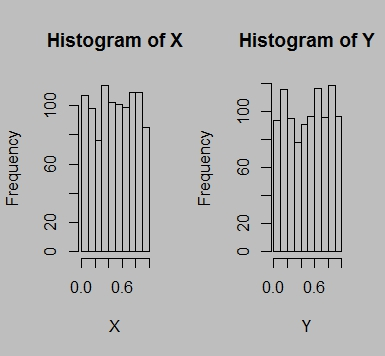
\includegraphics[scale=0.5]{fig1.jpeg} 
      \caption{ Plot to show f(x) is increasing for $x \leq \dfrac{(\alpha-1)}{((\alpha+\beta)-2)}$ and f(x) is decreasing for$x \geq \dfrac{(\alpha-1)}{((\alpha+\beta)-2)}$  \label{overflow}}
       \label{f(x) is maximum at 0.5}
\end{figure}

\textbf {R Code:}\\ 
\begin{verbatim}
a <- 2
b<- 2
xn <- seq(0,1,length=500)
f <-xn^(a-1)*(1-xn)^(b-1)/beta(a,b)
plot(x=c(0,1),y=c(0,10),xlab="x",ylab="f(x)")
lines(xn,f)
\end{verbatim}



\item The dominating density that can be used in the rejection sampling technique can be of Uniform distribution.\\


\item Implementing the acceptance and rejection algorithm for the parameter B($\alpha,\beta$)=(2,2)\\(Refer to Figure 6)
\begin{figure}[h]
     \centering
      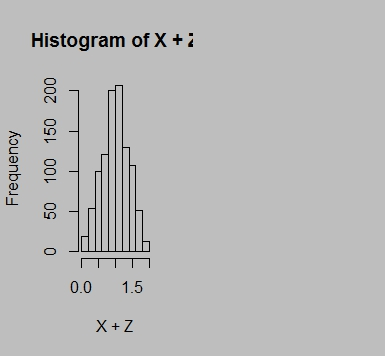
\includegraphics[scale=0.5]{fig2.jpeg}
       \caption{ Acceptance - Rejection algorithm $(\alpha,\beta)$=(2, 2) \label{overflow}}
         \label{Figure 6}
\end{figure}


\textbf {R Code :}\\
\begin{verbatim}
f <- function(x){
  fx <- x^(2-1)*(1-x)^(2-1)/beta(2,2)
}
num <- runif(500,0,1)
u <- runif(500,0,1)
t <- sapply(num,f)
ut <- u/t
hist(num[ut <=1], prob=T)
sum(ut<=1)/1000
\end{verbatim}

\textbf {Output:} The acceptance percentage is 40.7 percent\\

Implementing the rbeta function(Refer to Figure 7)
\begin{figure}[h]
      \centering
       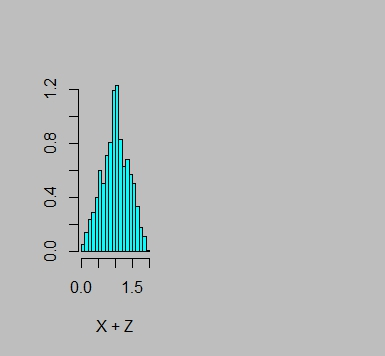
\includegraphics[scale=0.5]{fig3.jpeg}
        \caption{ Rbeta Histogram $(\alpha,\beta)$=(2, 2) \label{overflow}}
         \label{Figure 7}
\end{figure}

\begin{verbatim}
r<-rbeta(1,2,2)
ut1<-u/r
hist(num[ut1 <=1], prob=T)
\end{verbatim}



\end{enumerate}


\end{enumerate}

\end{document}
